\chapter{Finance and Time Series}

\section*{Why This Matters}

Financial services present unique challenges for transformer deployment that distinguish them from other AI applications. Non-stationary data distributions where patterns shift unpredictably. Regulatory requirements for explainability where every decision must be justified. Extreme latency constraints for high-frequency trading measured in microseconds. Severe consequences for prediction errors where mistakes cost millions. These constraints fundamentally shape architectural decisions, validation strategies, and deployment approaches.

The financial domain spans diverse applications with different technical requirements. Algorithmic trading requires sub-millisecond latency and robust handling of regime changes. Credit risk assessment demands explainability and fairness constraints. Anti-money laundering systems must balance detection accuracy against false positive burden while maintaining regulatory compliance. Fraud detection faces severe class imbalance with 99\% legitimate transactions. Each application requires specialized approaches that address its unique constraints.

Transformer architectures designed specifically for financial data address these challenges more effectively than standard models. Temporal Fusion Transformers handle multi-horizon forecasting with variable selection for time series. TabTransformers process categorical features more effectively than traditional gradient boosting for tabular data. Understanding when these specialized architectures justify their complexity—and when simpler approaches suffice—determines project success and cost efficiency.

This chapter examines three distinct financial applications: algorithmic trading with time series transformers, credit risk and fraud detection with tabular transformers, and anti-money laundering compliance systems. Each demonstrates different architectural choices, validation strategies, and deployment constraints that characterize production financial ML systems. The economic analysis reveals ROI ranging from 1--10× for e-discovery to 50--500× for AML compliance, with implementation costs from \$200,000 to \$50 million depending on scope and scale.

\section{Algorithmic Trading and Market Prediction}

Market prediction systems operate under constraints that distinguish them from other ML applications: non-stationary distributions where patterns shift unpredictably, microsecond latency requirements for high-frequency strategies, and direct financial consequences for every prediction error. These constraints shape every architectural and operational decision, from model selection through deployment infrastructure.

\subsection{Temporal Fusion Transformer Architecture}

The Temporal Fusion Transformer (TFT) addresses time series prediction through three specialized components: variable selection networks that identify relevant features from hundreds of candidates, temporal processing layers that capture patterns across multiple time scales, and multi-horizon prediction heads that forecast multiple time steps simultaneously. This architecture handles the complexity of financial time series more effectively than standard transformers designed for language.

\begin{figure}[htbp]
\centering
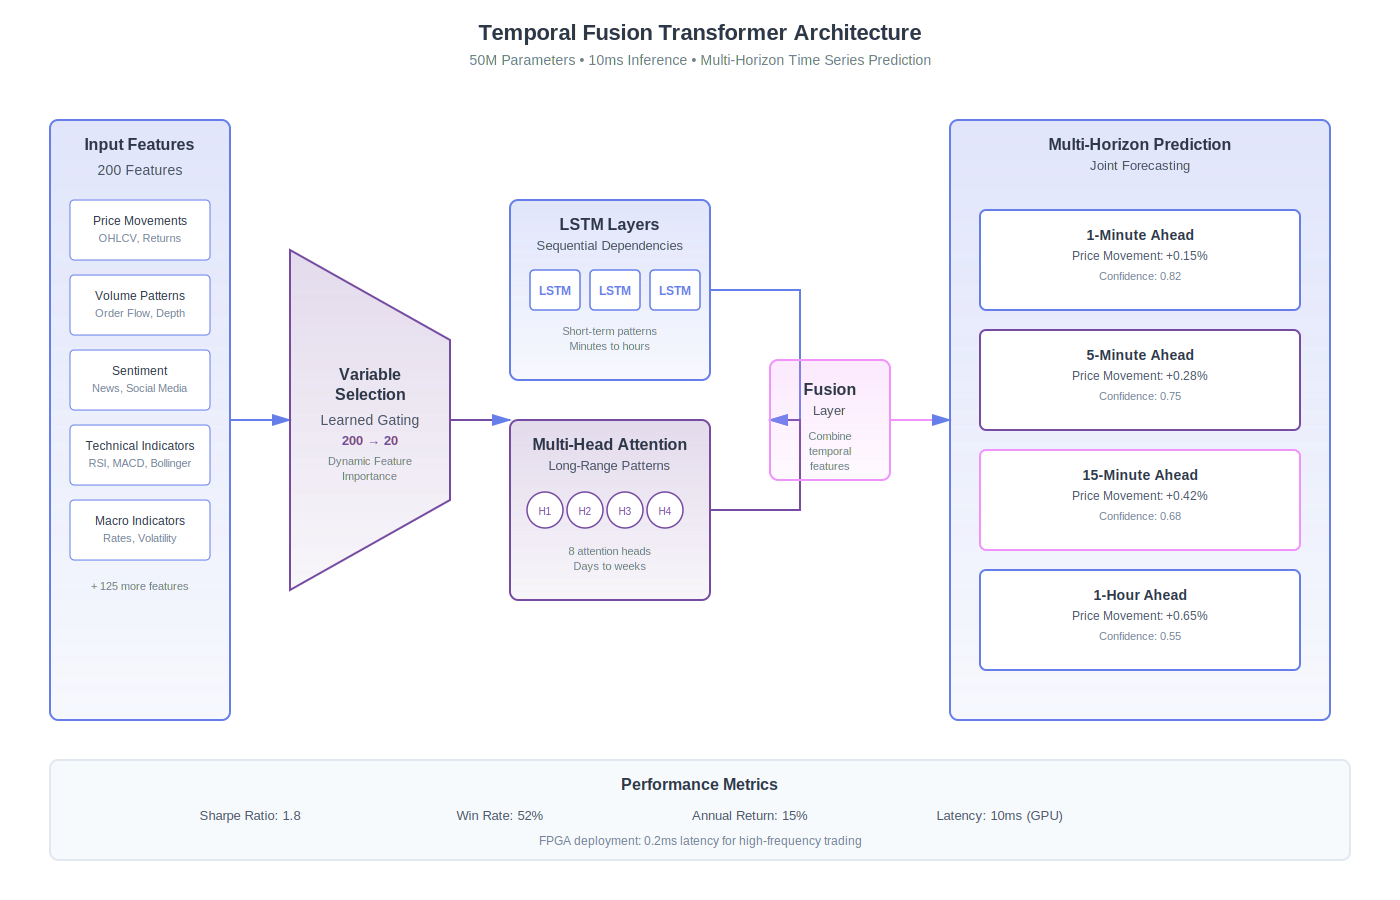
\includegraphics[width=0.95\textwidth]{chapters/diagrams/chapter14_tft_architecture_a1b2c3d4.pdf}
\caption{Temporal Fusion Transformer architecture showing variable selection network (200 to 20 features), LSTM layers for sequential dependencies, multi-head attention for long-range patterns, and multi-horizon prediction heads generating forecasts at 1-minute, 5-minute, 15-minute, and 1-hour horizons}
\label{fig:tft_architecture}
\end{figure}

Variable selection operates through learned gating mechanisms that weight input features dynamically. Given 200 potential features—price movements, volume patterns, order book depth, sentiment indicators, macroeconomic variables—the network learns to emphasize the 20 most predictive features for current market conditions. This selection adapts over time as market regimes change, unlike fixed feature engineering that requires manual updates.

The temporal processing architecture combines LSTM layers for sequential dependencies with multi-head attention for long-range patterns. LSTM components capture short-term momentum and mean reversion patterns spanning minutes to hours. Attention mechanisms identify longer-term relationships across days or weeks, such as earnings cycles or macroeconomic announcements. This hybrid approach handles both high-frequency patterns and structural market dynamics.

Multi-horizon prediction generates forecasts for multiple future time steps simultaneously—predicting price movements at 1 minute, 5 minutes, 15 minutes, and 1 hour ahead in a single forward pass. This joint prediction captures relationships between different time horizons more effectively than training separate models. A 50-million parameter TFT model processes 200 features and generates 4-horizon predictions in approximately 10 milliseconds on GPU hardware.

\subsection{Walk-Forward Validation and Lookahead Bias}

Financial time series validation requires walk-forward testing that simulates actual trading conditions. Standard k-fold cross-validation introduces lookahead bias—training on future data to predict the past—that produces misleadingly optimistic results. Walk-forward validation trains on historical data, tests on subsequent periods, then retrains including the test period before advancing to the next window.

A typical walk-forward schedule trains on 2 years of data, tests on 1 month, then advances the window by 1 month. This process repeats across the entire historical period, generating performance metrics that reflect realistic trading conditions. For a 5-year backtest with monthly retraining, this requires 60 separate training runs. At 4 GPU-hours per training run on A100 hardware, the validation process consumes 240 GPU-hours at approximately \$600 in compute costs.

The computational expense increases substantially when optimizing hyperparameters. Testing 10 hyperparameter configurations across the same 60-month walk-forward schedule requires 2,400 GPU-hours—roughly \$6,000 in compute costs. This expense explains why financial ML teams typically limit hyperparameter search to critical parameters like learning rate, attention heads, and regularization strength, while fixing architectural choices based on domain knowledge.

Lookahead bias detection requires careful data pipeline design. Features must use only information available at prediction time. A common error: calculating technical indicators using the entire day's data when predicting intraday movements. Proper implementation calculates indicators using only data through the prediction timestamp. Similarly, fundamental data like earnings reports must use announcement dates, not report dates, to avoid incorporating information unavailable to traders.

\subsection{Adversarial Training for Non-Stationarity}

Financial markets exhibit non-stationarity—statistical properties change over time as market regimes shift. A model trained on low-volatility periods performs poorly during market stress. Adversarial training improves robustness by exposing the model to artificially perturbed data that simulates regime changes.

The adversarial training process generates synthetic examples by applying small perturbations to input features that maximize prediction error. These adversarial examples represent market conditions the model finds challenging—typically regime boundaries where patterns shift. Training on both original and adversarial examples improves performance during actual regime changes, though at the cost of slightly reduced performance during stable periods.

Implementation adds 30-40\% to training time, as generating adversarial examples requires additional forward and backward passes. For the 240 GPU-hour walk-forward validation, adversarial training increases compute to approximately 330 GPU-hours—roughly \$825 in costs. This investment proves worthwhile for strategies deployed during volatile periods, where regime robustness determines profitability.

\subsection{FPGA Deployment for Low Latency}

High-frequency trading strategies require sub-millisecond latency from signal generation to order execution. GPU inference, while fast for batch processing, introduces 5-10 milliseconds of latency from data transfer and kernel launch overhead. FPGA deployment achieves 0.2 millisecond latency by implementing the model directly in hardware logic.

FPGA implementation requires converting the trained model to fixed-point arithmetic and synthesizing neural network operations as hardware circuits. This conversion process, performed by specialized tools like Xilinx Vitis AI, takes 2-3 weeks of engineering time and requires careful validation to ensure numerical accuracy matches the original floating-point model. Quantization to 8-bit or 16-bit fixed-point typically introduces less than 1\% accuracy degradation for financial models.

Hardware costs differ substantially from GPU deployment. A high-end FPGA card costs \$5,000-\$10,000 with negligible operating costs beyond power consumption. A comparable GPU costs \$10,000-\$15,000 with similar power requirements. The FPGA advantage lies in latency, not cost or throughput. For strategies where microseconds matter—market making, arbitrage, momentum trading—FPGA deployment justifies the engineering investment. For longer-horizon strategies, GPU inference suffices.

\subsection{Ensemble Methods and Confidence Intervals}

Financial prediction systems typically deploy ensembles of 5-10 models trained with different random seeds, architectures, or data samples. Ensemble predictions average individual model outputs, while prediction variance across ensemble members provides confidence intervals. These confidence intervals inform position sizing and risk management decisions.

A prediction with narrow confidence intervals—high agreement across ensemble members—justifies larger position sizes. Wide confidence intervals indicate model uncertainty, suggesting smaller positions or avoiding the trade entirely. This risk-aware approach improves risk-adjusted returns substantially. A strategy with 52\% win rate and 1.8 Sharpe ratio using confidence-based position sizing might achieve only 1.2 Sharpe ratio with fixed position sizes.

Ensemble deployment multiplies inference costs by the number of models. A 5-model ensemble requires 5× the compute resources of a single model. For FPGA deployment at 0.2 milliseconds per model, a 5-model ensemble completes in 1 millisecond—still acceptable for high-frequency strategies. For GPU deployment, ensemble inference takes 50 milliseconds, limiting applicability to lower-frequency strategies.

\subsection{Performance Metrics and Economics}

Trading strategy performance uses risk-adjusted metrics rather than raw returns. Sharpe ratio—excess return divided by return volatility—measures risk-adjusted performance. A Sharpe ratio of 1.8 indicates the strategy generates 1.8 units of excess return per unit of risk, considered strong performance for quantitative strategies. Win rate—percentage of profitable trades—provides additional context. A 52\% win rate with proper risk management generates consistent profits.

Annual returns depend on capital allocation and leverage. A strategy generating 15\% annual return on \$10 million capital produces \$1.5 million in profits. Infrastructure costs include compute resources, data feeds, and operational expenses. For the TFT-based strategy described:

\begin{itemize}
\item Training and validation: \$6,000 annually (monthly retraining with hyperparameter optimization)
\item FPGA hardware: \$50,000 initial investment, \$5,000 annual maintenance
\item Market data feeds: \$200,000 annually (real-time tick data, order book depth)
\item Operational costs: \$500,000 annually (infrastructure, monitoring, risk management)
\end{itemize}

Total annual costs approximate \$800,000. With \$1.5 million in profits, net return reaches \$700,000 or 7\% on capital—attractive for institutional investors when considering risk-adjusted characteristics.

\section{Credit Risk Assessment and Fraud Detection}

Credit risk and fraud detection systems process structured tabular data with hundreds of features, many categorical. Traditional gradient boosting methods like XGBoost excel at this task, but transformer-based approaches offer advantages for categorical feature handling and transfer learning from related tasks. Understanding when transformers justify their complexity requires analyzing the specific characteristics of the prediction problem.

\subsection{TabTransformer Architecture}

TabTransformer adapts transformer architecture for tabular data by treating categorical features as tokens and applying self-attention to learn feature interactions. Continuous features pass through standard feed-forward layers, while categorical features receive learned embeddings that capture semantic relationships. This approach handles high-cardinality categorical features—merchant IDs, product categories, geographic regions—more effectively than one-hot encoding or target encoding used by tree-based methods.

\begin{figure}[htbp]
\centering
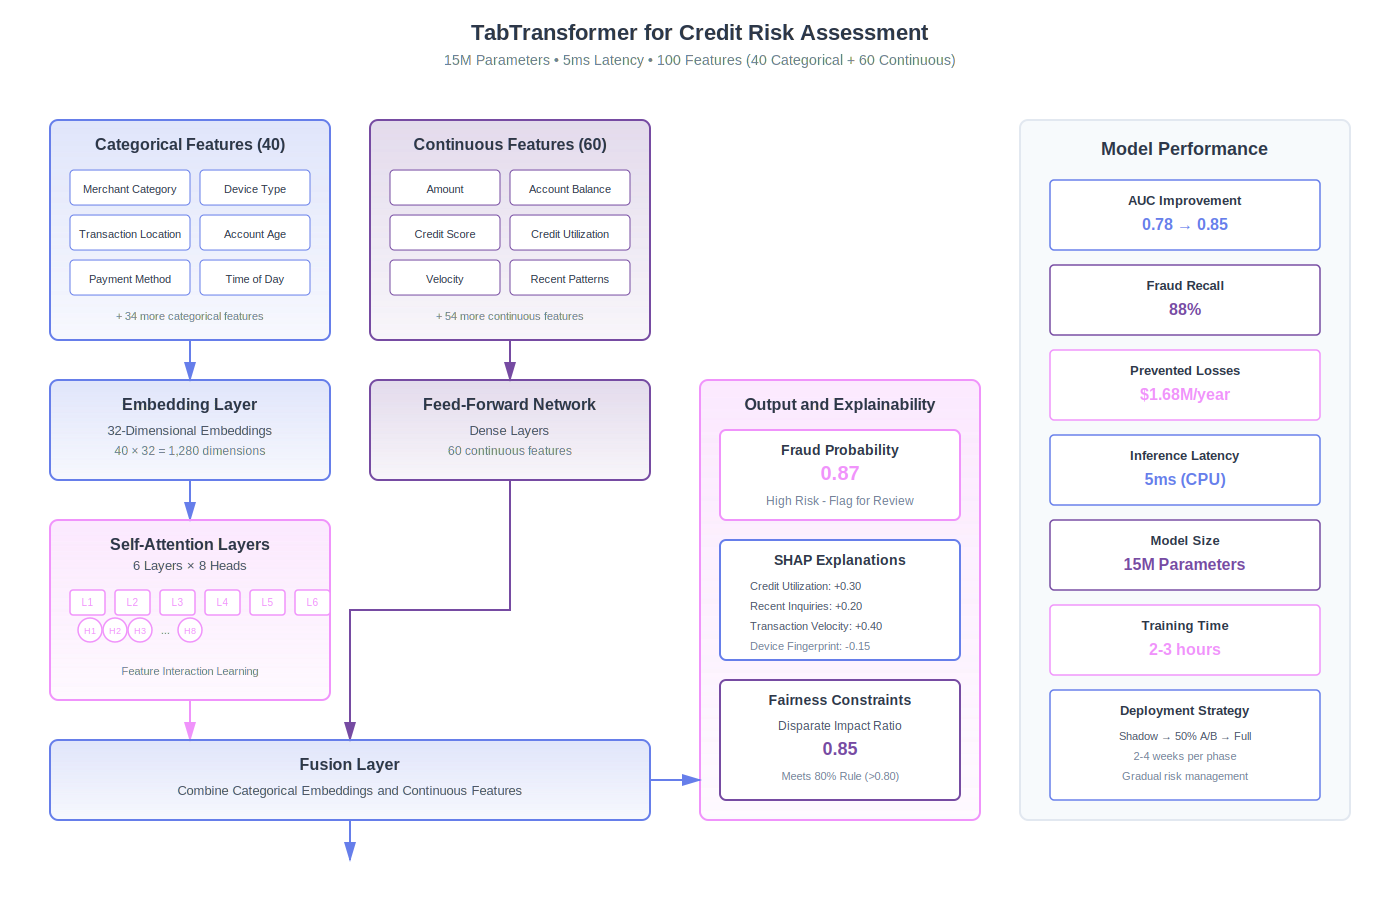
\includegraphics[width=0.95\textwidth]{chapters/diagrams/chapter14_credit_risk_model_e5f6g7h8.pdf}
\caption{TabTransformer architecture for credit risk assessment processing 40 categorical features through embedding and self-attention layers (6 layers, 8 heads) and 60 continuous features through feed-forward networks, with SHAP explainability and fairness constraint monitoring}
\label{fig:credit_risk_model}
\end{figure}

The architecture processes a credit application with 100 features: 40 categorical (merchant category, transaction location, device type, account age bucket) and 60 continuous (transaction amount, account balance, recent transaction patterns, credit utilization). Categorical features receive 32-dimensional embeddings, creating a 40×32 embedding matrix. Self-attention layers learn which categorical features interact—for example, that certain merchant categories combined with specific geographic regions indicate elevated fraud risk.

A typical TabTransformer for credit risk uses 6 attention layers with 8 heads each, totaling approximately 15 million parameters. This model size enables training on a single GPU in 2-3 hours using 1 million historical transactions. Inference latency reaches 5 milliseconds per prediction on CPU hardware, acceptable for real-time credit decisions that tolerate 100-200 millisecond total latency including data retrieval and business logic.

\subsection{Traditional and Alternative Data Features}

Credit risk models combine traditional credit bureau data with alternative data sources that provide additional signal. Traditional features include credit score, payment history, credit utilization, account age, and recent inquiries. Alternative data encompasses transaction patterns, device fingerprints, behavioral biometrics, social network indicators, and employment verification data.

Alternative data improves prediction accuracy for thin-file applicants—individuals with limited credit history—where traditional features provide insufficient signal. A model using only traditional features might achieve 0.78 AUC (area under ROC curve) on thin-file applicants, while adding alternative data improves AUC to 0.85. This 7-point improvement translates to substantial business value: approving more creditworthy applicants while maintaining fraud rates.

Feature engineering for alternative data requires domain expertise. Raw transaction data—timestamps, amounts, merchants—provides limited signal. Engineered features capture behavioral patterns: transaction velocity (transactions per day), amount distributions (mean, variance, percentiles), merchant diversity (unique merchants per month), and temporal patterns (weekday versus weekend spending). These engineered features often provide more signal than raw data.

\subsection{Class Imbalance and Focal Loss}

Fraud detection faces severe class imbalance: typically 1\% of transactions are fraudulent, 99\% legitimate. Standard cross-entropy loss trains models that predict "legitimate" for all transactions, achieving 99\% accuracy while catching zero fraud. Addressing class imbalance requires specialized loss functions and sampling strategies.

Focal loss down-weights easy examples—legitimate transactions the model predicts confidently—while emphasizing hard examples—fraudulent transactions the model finds challenging. The loss function includes a focusing parameter that controls this emphasis. For fraud detection with 1\% positive rate, focal loss with focusing parameter 2.0 typically improves fraud recall from 60\% to 88\% while maintaining precision above 80\%.

SMOTE (Synthetic Minority Over-sampling Technique) generates synthetic fraud examples by interpolating between existing fraud cases in feature space. This oversampling balances the training set, improving model sensitivity to fraud patterns. However, SMOTE can introduce artifacts if synthetic examples fall in regions of feature space that don't represent realistic fraud. Careful validation ensures synthetic examples improve rather than degrade model performance.

Combined approaches—focal loss during training with SMOTE oversampling—typically outperform either technique alone. Implementation requires careful hyperparameter tuning: SMOTE oversampling ratio (2:1, 3:1, or 5:1 fraud to legitimate), focal loss focusing parameter (1.5, 2.0, or 2.5), and class weights. Grid search across these parameters adds 20-30\% to training time but substantially improves fraud detection performance.

\subsection{Explainability and SHAP Values}

Financial services regulations require explainability for credit decisions—applicants must receive specific reasons for denial. SHAP (SHapley Additive exPlanations) values provide feature-level explanations by calculating each feature's contribution to individual predictions. For a denied application, SHAP values might indicate that high credit utilization contributed +0.3 to the fraud score, recent inquiries added +0.2, and unusual transaction velocity added +0.4.

Computing SHAP values requires multiple model evaluations per prediction—typically 100-500 evaluations to estimate feature contributions accurately. This computational cost makes SHAP impractical for real-time scoring of all transactions. Production systems compute SHAP values only for denied applications or flagged transactions requiring review, reducing the explanation workload to 1-2\% of total predictions.

SHAP values also enable model debugging and fairness analysis. Examining SHAP value distributions across demographic groups reveals whether the model relies on protected attributes or their proxies. If SHAP analysis shows that geographic features contribute disproportionately to denials for certain demographic groups, this indicates potential fairness issues requiring model adjustment or feature removal.

\subsection{Fairness Constraints and Disparate Impact}

Credit models must satisfy fairness constraints that limit disparate impact across demographic groups. Disparate impact measures the ratio of approval rates between groups—for example, approval rate for minority applicants divided by approval rate for majority applicants. Regulatory guidance typically requires this ratio to exceed 0.8 (the "80\% rule"), meaning minority approval rates must reach at least 80\% of majority approval rates.

Enforcing fairness constraints during training requires specialized optimization techniques. Post-processing approaches adjust decision thresholds separately for each group to achieve desired approval rate ratios. In-processing methods incorporate fairness constraints directly into the loss function, penalizing predictions that increase disparate impact. These techniques typically reduce overall model accuracy by 1-2 percentage points while ensuring fairness requirements.

Fairness-accuracy trade-offs require business judgment. A model achieving 0.87 AUC with 0.85 disparate impact ratio might be preferable to a model with 0.88 AUC and 0.75 disparate impact ratio, despite lower accuracy. The fairness improvement reduces regulatory risk and reputational harm, while the accuracy decrease has minimal business impact. Quantifying these trade-offs requires collaboration between ML teams, legal counsel, and business stakeholders.

\subsection{A/B Testing and Gradual Rollout}

Production deployment of credit models follows a gradual rollout strategy that manages risk while gathering performance data. The rollout typically progresses through three phases: shadow mode, partial deployment, and full deployment. Each phase validates model performance before expanding scope.

Shadow mode runs the new model alongside the existing production model, generating predictions without affecting decisions. This phase validates that the model performs as expected on production data, identifies data pipeline issues, and establishes baseline performance metrics. Shadow mode typically runs for 2-4 weeks, processing all production traffic while making zero business impact.

Partial deployment routes a percentage of traffic—typically 10-20\% initially, expanding to 50\%—to the new model while the existing model handles remaining traffic. This A/B test measures business impact: approval rates, fraud rates, revenue, and customer satisfaction. Statistical significance requires 2-4 weeks depending on traffic volume. For a system processing 100,000 applications daily, 2 weeks of 50\% traffic provides sufficient data to detect 0.5 percentage point differences in fraud rates with 95\% confidence.

Full deployment occurs only after partial deployment demonstrates improved or equivalent performance across all metrics. Even after full deployment, the previous model remains available for rapid rollback if issues emerge. This cautious approach prevents catastrophic failures that could result from deploying an untested model to all traffic immediately.

\subsection{Business Impact and Economics}

Credit risk model improvements translate directly to business value through increased approvals of creditworthy applicants and reduced fraud losses. A model improving AUC from 0.78 to 0.85 enables approving an additional 5\% of applicants while maintaining the same fraud rate, or maintaining the same approval rate while reducing fraud by 30\%.

For a lender processing 1 million applications annually with 60\% approval rate and 2\% fraud rate on approved applications, the business impact calculation proceeds as follows. The baseline system approves 600,000 applications with 12,000 fraud cases. At \$500 average loss per fraud case, annual fraud losses reach \$6 million. The improved model with 88\% fraud recall (up from 60\%) catches 10,560 fraud cases instead of 7,200, preventing an additional 3,360 fraud cases worth \$1.68 million annually.

Alternatively, maintaining the same fraud rate while increasing approvals generates revenue from additional customers. Approving 5\% more applicants—30,000 additional approvals—generates revenue from interest and fees. At \$200 annual revenue per customer, this produces \$6 million in additional annual revenue. The optimal strategy depends on business priorities: growth versus risk management.

Model development and operational costs include:

\begin{itemize}
\item Initial development: \$200,000 (3 months, 2 ML engineers, 1 data scientist)
\item Training infrastructure: \$10,000 annually (GPU compute for monthly retraining)
\item Inference infrastructure: \$50,000 annually (CPU servers for real-time scoring)
\item Monitoring and maintenance: \$100,000 annually (1 ML engineer part-time)
\item Data costs: \$500,000 annually (alternative data sources, credit bureau data)
\end{itemize}

Total annual costs approximate \$660,000 after initial development. With \$1.68 million in prevented fraud losses or \$6 million in additional revenue, the ROI justifies the investment substantially. The payback period for initial development costs reaches 2-3 months.

\section{Portfolio Optimization and Asset Allocation}

\subsection{Modern Portfolio Theory and Efficient Frontier}

Portfolio optimization determines optimal allocation of capital across multiple assets to balance return and risk. Traditional approaches use Markowitz mean-variance optimization, allocating weights to minimize portfolio volatility for a given expected return, or maximize return for a given volatility constraint.

The efficient frontier represents the set of optimal portfolios dominating all others—no other portfolio achieves higher return for the same risk or lower risk for the same return. Optimal portfolio allocation typically involves 10-50 different assets, with weights changing monthly as return expectations and correlations evolve.

Constrained optimization handles real-world constraints: sector exposure limits (maximum 30\% in technology), concentration limits (maximum 10\% per single stock), leverage limits, and dividend yield requirements. These constraints often have greater impact on performance than the optimization algorithm itself.

\subsection{Machine Learning Improvements Over Traditional Approaches}

Traditional mean-variance optimization struggles with three problems: correlation estimates are unstable and highly uncertain, expected returns are impossible to forecast accurately, and constraints are hard-coded and inflexible.

Machine learning approaches address these limitations through several mechanisms. Correlation prediction models learn which correlations are stable and which time-varying. During market stress, normally low-correlation assets become highly correlated—a phenomenon that traditional approaches fail to anticipate.

Return forecasting uses models that predict returns conditional on market regime, valuations, sentiment, and other factors. These dynamic return forecasts improve portfolio optimization compared to assuming constant expected returns.

Constraint adaptation allows models to learn which constraints bind under different market conditions. During high-volatility periods, leverage constraints should tighten; during stable periods, they can loosen.

Regime-aware optimization recognizes that different optimization approaches suit different market regimes. During normal markets, mean-variance optimization works well. During stress periods, risk-parity or equal-weight approaches perform better. Models can identify the current regime and select appropriate optimization strategies.

Expected improvement over traditional approaches ranges from 0.5-1.5\% annual return improvement. For a \$1 billion portfolio, this translates to \$5-15 million annually.

\subsection{Rebalancing and Transaction Costs}

Portfolio rebalancing—adjusting weights back to optimal allocations—occurs periodically. Monthly rebalancing keeps weights close to optimal but incurs transaction costs. Quarterly or annual rebalancing reduces transaction costs at the expense of drift from optimal allocations.

Transaction costs include bid-ask spreads, commissions, and market impact of large trades. For a \$1 billion portfolio rebalancing 30\% of holdings monthly, transaction costs approximate 0.05-0.10\% of portfolio value, or \$500,000-1,000,000 annually. This transaction cost must be justified by performance improvements.

Multi-period portfolio optimization considers transaction costs explicitly, finding allocations that balance expected return against trading costs. Models can identify when rebalancing is worthwhile—when return improvement exceeds transaction costs—and when to skip rebalancing.

\section{Customer Lifetime Value and Churn Prediction}

\subsection{Customer Lifetime Value Prediction}

Customer lifetime value (CLV)—total profit a customer will generate over their relationship with the company—drives customer acquisition and retention decisions. Acquisition costs justify spending up to 30-50\% of expected CLV to acquire a customer. Retention spending should increase with CLV.

Predicting CLV from customer characteristics, product usage, and account history enables several strategic capabilities. Acquisition targeting focuses acquisition spending on customer segments with high CLV—mobile customers might have 3× CLV of web-only customers. Retention prioritization allocates more resources to retaining high-CLV customers and less to low-CLV customers. Product recommendations align with customer preferences and profitability, recommending higher-margin products to customers most likely to purchase them. Lifecycle management enables stage-specific actions for different customer phases: new customers need onboarding, mature customers need expansion opportunities, at-risk customers need retention outreach.

CLV models typically use gradient boosted models or neural networks to predict expected profit from historical customer data. Features include customer demographics, account tenure, product holdings, transaction volumes, interaction history, and service quality metrics.

\subsection{Churn Prediction}

Churn prediction identifies customers likely to leave, enabling proactive retention outreach. For subscription businesses, even 5\% improvement in churn rates translates to 15-25\% revenue improvement through compounding over time.

Churn prediction models predict the probability that a customer will leave within a specified period—next month or next quarter. Customers with high churn risk receive targeted retention offers: service discounts, exclusive features, or personal support.

High-value customers warrant more aggressive retention spending. A model predicting 40\% churn risk for a \$10,000/month customer justifies offering \$2,000/month discounts—keeping the customer is worth \$8,000/month in retained revenue. For a \$100/month customer, the same intervention is not justified.

Churn models inform product development by identifying which feature gaps drive churn. If customers leaving use certain features less frequently, product improvements in those areas would reduce churn.

\subsection{Cross-Sell and Upsell Propensity}

Propensity models predict customer likelihood to purchase specific products. Product-specific models predict purchase probability for a particular product, such as an enterprise support add-on. General propensity models predict likelihood to buy any higher-value product.

Models identify which customer segments respond best to which offers. Email campaigns targeting customers most likely to purchase specific products achieve much higher response rates than mass marketing.

Timing models predict when customers are most receptive to offers. Recent product switchers might be more open to upgrade offers. Customers who just had negative support interactions might be more responsive to win-back offers.

\subsection{Economics and Implementation}

For a SaaS company with 100,000 customers averaging \$200 monthly (\$24 million annual revenue), the business impact breaks down as follows.

Churn improvement from reducing 5\% churn to 4\% through improved retention retains an additional \$2.4 million in revenue annually. At \$1,000 cost per retained customer, this generates \$1.4 million net value.

CLV improvement through more accurate prediction improves acquisition targeting and retention prioritization. Better targeting improves acquisition ROI by 10-20\%, translating to \$2-4 million annual value for acquisition budgets.

Implementation requires integrating CLV and churn models with customer success and marketing systems. Models score all customers weekly, generating lists of high-churn-risk, high-CLV customers for proactive outreach. Integration typically costs \$50,000-100,000; annual system costs approximate \$100,000.

With \$3-5 million annual value and \$100,000 annual costs, ROI reaches 30-50×.

\section{Feature Engineering and Data Quality}

\subsection{Data Quality and Missing Data}

Financial data quality varies dramatically. Real-time trading data is clean and complete. Alternative data sources like satellite imagery or credit card data have inconsistent coverage and gaps. Feature engineering and quality assurance consume 40-60\% of financial ML project effort.

Missing data requires careful handling. Simple approaches like mean imputation introduce bias. Domain-aware approaches—recognizing that missing volume data implies a liquidity event—preserve information better. Multiple imputation provides uncertainty estimates for downstream analysis.

Outliers require investigation rather than automatic removal. A 50\% stock price move is unusual but legitimate, reflecting an earnings surprise. A 5,000\% move is likely a data error. Domain expertise distinguishes legitimate outliers from errors.

\subsection{Feature Engineering from Raw Data}

Raw financial data—OHLCV (open, high, low, close, volume)—provides limited predictive signal. Feature engineering constructs more predictive variables.

Technical indicators like moving averages capture trend, RSI measures momentum, and Bollinger Bands indicate volatility. These indicators are computed from only historical data through the prediction timestamp, avoiding lookahead bias.

Market microstructure features including order book depth, bid-ask spreads, and order imbalance indicate market stress and short-term price direction.

Temporal features capture time of day, day of week, proximity to market opens and closes, and proximity to earnings dates, revealing seasonal and event-driven patterns.

Cross-sectional features measure relative performance—stock performance relative to sector—correlation changes, and price momentum relative to peers.

Proper feature engineering requires deep financial domain knowledge. Implementing features incorrectly, such as introducing lookahead bias in indicators, produces results that pass validation but fail in production.

\subsection{Feature Selection and Dimensionality}

Financial models often have 500+ features. Not all are predictive; many are noisy or redundant. Feature selection reduces noise and improves generalization.

Correlation analysis identifies redundant features. If two features are 0.95 correlated, they provide similar information and one can be removed. However, intentional correlation—different technical indicators measuring trend—can be valuable.

Importance-based selection ranks features by their contribution to predictions. Tree-based models provide built-in importance measures. Neural networks require SHAP or other explainability techniques. Selecting top-K features, such as the top 50 of 500, significantly reduces model complexity while often improving generalization.

Stability analysis measures whether feature importance changes over time. Features that are critical during some periods but irrelevant during others require regime-specific feature selection.

\section{Model Monitoring and Governance}

\subsection{Performance Monitoring and Degradation}

Deployed financial models degrade over time as market regimes change and data distributions shift. Regular monitoring detects degradation before it causes significant losses.

Performance metrics tracked continuously include prediction accuracy, Sharpe ratio, win rate, and fraud detection recall and precision. Alerts trigger when metrics fall below thresholds. For example, if fraud detection recall drops below 80\%, the system alerts for model investigation.

Performance decomposition identifies where degradation occurs. Degradation might be concentrated in certain market regimes like high-volatility periods, certain customer segments such as new account holders, or certain time periods like recent months. Targeted analysis identifies root causes.

\subsection{Data Drift and Concept Drift}

Data drift occurs when input distributions change, such as when an economic recession changes customer credit profiles. Concept drift occurs when relationships change, such as when a pandemic changes correlation between sectors.

Drift detection uses statistical tests to identify when distributions diverge significantly from training data. Sudden drift, like pandemic onset, requires immediate model retraining. Gradual drift, like slow economic deterioration, allows scheduled retraining.

\subsection{Retraining Frequency and Triggers}

Retraining frequency balances model freshness against computational cost. For algorithmic trading, daily or weekly retraining adapts to market changes. For credit models, monthly retraining suffices; annual retraining is insufficient.

Event-based retraining triggers when performance falls below thresholds, significant data drift is detected, major market events occur like crashes or policy changes, or regulatory changes require model adjustment.

Scheduled retraining ensures regular updates even if no specific event triggers retraining.

\subsection{Model Versioning and Governance}

Managing multiple model versions is essential for production systems. Key practices include version control to track all model code, training data, hyperparameters, and results, enabling reproduction of any model version.

Approval processes move models through stages—development, validation, production—with approval at each stage. Production models have clear ownership and governance.

Audit trails document when models were trained, on what data, with what performance, and when deployed, enabling investigation of model decisions.

Rollback capability maintains the ability to quickly revert to previous models if current models cause issues.

\section{When to Use Specialized Architectures}

\subsection{TabTransformer vs. XGBoost}

For credit risk prediction, does TabTransformer justify its complexity compared to XGBoost? A typical comparison reveals the trade-offs.

In terms of accuracy, TabTransformer achieves 0.85 AUC while XGBoost achieves 0.833 AUC. The 1.7 percentage point improvement represents reduced fraud. For a lender processing 1 million applications, this improvement prevents approximately 1,700 additional fraud cases at \$500 loss each, equaling \$850,000 annual value.

Development cost for TabTransformer requires 3 months with 2 engineers and 1 data scientist, totaling \$200,000. XGBoost requires 6 weeks at \$100,000. Additional development cost: \$100,000.

Operational cost for TabTransformer requires GPU infrastructure at \$10,000 annually. XGBoost requires CPU infrastructure at \$2,000 annually. Additional operational cost: \$8,000 annually.

ROI calculation: \$850,000 fraud prevention minus \$100,000 additional development minus \$8,000 annual operational cost equals \$742,000 annual net value. This ROI justifies TabTransformer investment.

However, if fraud improvement were only 0.5 percentage points (\$250,000 annual value), the \$100,000 development investment would not be justified. The decision depends on the actual accuracy improvement, which requires empirical validation.

\subsection{Temporal Fusion Transformer vs. ARIMA}

For stock price forecasting, does TFT justify its complexity compared to statistical approaches?

In terms of accuracy, TFT achieves 0.52 Sharpe ratio while ARIMA achieves 0.38 Sharpe ratio. The improvement represents higher risk-adjusted returns.

Development cost for TFT requires 4 months with 2 engineers, totaling \$150,000. ARIMA requires 2 weeks at \$10,000. Additional cost: \$140,000.

Operational cost for TFT requires GPU infrastructure at \$50,000 annually. ARIMA requires CPU at \$5,000. Additional cost: \$45,000.

Strategy value: For \$10 million capital, TFT Sharpe of 0.52 generates approximately \$1.2 million in annual returns. ARIMA generates approximately \$900,000. Additional value: \$300,000.

ROI calculation: \$300,000 annual returns minus \$140,000 development minus \$45,000 operational equals \$115,000 annual net value. This ROI justifies TFT investment.

However, this assumes the Sharpe ratio improvement actually occurs in production. Backtests often overestimate performance due to lookahead bias and overfitting. If production performance shows only 0.05 Sharpe improvement instead of 0.14, the value drops to \$50,000 annually, which barely justifies investment.

\subsection{The Importance of Empirical Validation}

The decision to deploy specialized architectures must be based on empirical validation, not theoretical arguments. A model that achieves 0.01 percentage point improvement in backtests but fails in production provides no value despite theoretical justification.

Key validation principles include walk-forward validation that simulates production conditions, out-of-sample validation on completely held-out data, pilot deployment before full rollout, and realistic performance estimation accounting for overfitting risk.

\section{Regulatory Framework and Compliance}

\subsection{Model Risk Management}

Federal Reserve guidance (SR 11-7) establishes Model Risk Management requirements for large financial institutions. Key requirements include model validation through independent validation before and after deployment, including performance monitoring and stress testing.

Model governance requires clear policies, procedures, and oversight. Models must be approved before deployment and re-approved periodically.

Risk management assesses and manages risks from model errors. Institutions must establish thresholds triggering model review or replacement.

\subsection{Stress Testing and CCAR/DFAST}

Comprehensive Capital Analysis and Review (CCAR) and Dodd-Frank Act Stress Testing (DFAST) require large banks to demonstrate capital adequacy under adverse scenarios. Models predict losses under various economic scenarios including recession, market crash, and unemployment spike.

These stress testing models often use machine learning to map economic scenarios to specific outcomes. Credit loss models, trading loss models, and operational risk models all require scenario analysis.

\subsection{Fair Lending Compliance}

The Equal Credit Opportunity Act requires that credit models not discriminate based on protected characteristics. Fair Lending exams scrutinize credit models for disparate impact. Models must demonstrate that differences in outcomes reflect legitimate creditworthiness factors, not protected characteristics or proxies.

\subsection{Market Abuse and Algorithmic Trading}

The Securities and Exchange Commission (SEC) and regulatory bodies scrutinize algorithmic trading for market manipulation. Models must be able to explain trading decisions and demonstrate that they do not engage in prohibited practices like spoofing, layering, or pump-and-dump schemes.

\section{Key Insights}

\textbf{Specialized Architectures Address Specific Data Characteristics}: Temporal Fusion Transformers for time series with variable selection and multi-horizon prediction. TabTransformers for tabular data with categorical features. Understanding whether data characteristics justify architectural complexity determines project success.

\textbf{Walk-Forward Validation Is Essential for Financial Applications}: Standard cross-validation introduces lookahead bias producing misleadingly optimistic results. Walk-forward testing correctly simulates production conditions but requires substantial compute. The \$600-6,000 validation cost for backtests is necessary investment, not optional optimization.

\textbf{Non-Stationarity Requires Adaptive Approaches}: Fixed models degrade as market regimes change. Adversarial training improves robustness. Frequent retraining adapts to changing conditions. Ensemble methods provide confidence intervals informing risk management.

\textbf{Latency Requirements Drive Deployment Architecture}: Sub-millisecond requirements drive FPGA deployment despite 2-3 weeks engineering effort. Millisecond-scale requirements use GPUs. Second-scale requirements use CPU. Understanding latency requirements before architecture selection prevents costly redesign.

\textbf{Class Imbalance Requires Specialized Techniques}: Fraud detection with 1\% positive rate requires focal loss and SMOTE. Standard cross-entropy loss produces models predicting "legitimate" for all transactions, achieving accuracy while catching zero fraud.

\textbf{Regulatory Requirements Are Non-Negotiable}: Fair lending compliance, model risk management, and stress testing requirements cannot be postponed. Compliance architecture decisions affect model design and deployment.

\textbf{Economic Justification Must Be Based on Empirical Validation}: Decisions to deploy specialized architectures must rest on production performance, not backtests. Overfitting in backtests produces overoptimistic estimates. Pilot deployment before full rollout validates assumptions.
